\documentclass[11pt, oneside]{article} 
\usepackage{geometry}
\geometry{letterpaper} 
\usepackage{graphicx}
	
\usepackage{amssymb}
\usepackage{amsmath}
\usepackage{parskip}
\usepackage{color}
\usepackage{hyperref}

\graphicspath{{/Users/telliott/Github/figures/}}
% \begin{center} \includegraphics [scale=0.4] {gauss3.png} \end{center}

\title{Law of cosines}
\date{}

\begin{document}
\maketitle
\Large

%[my-super-duper-separator]

\label{sec:Law_of_cosines}

\subsection*{Law of cosines}

Designate the lengths of a triangle's sides as $a,b,c$ and the angle between sides $a$ and $b$ as $C$ (because it is opposite side $c$).  The law of cosines says that

\begin{center} 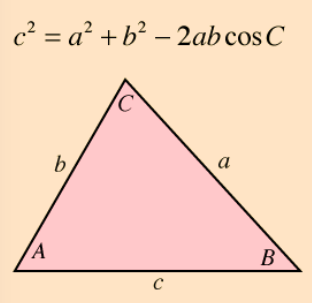
\includegraphics [scale=0.5] {cosine_law.png} \end{center}

\[ c^2 = a^2 + b^2 - 2 a b \cos C \]

Lockhart calls this the "generalized" Pythagorean theorem.  We can view the term $-2ab \cos C$ as a correction term which disappears in the case where $\angle C$ is 90 degrees.

If $\angle C$ were a right angle then we would have that
\[ c^2 = a^2 + b^2 \]
but since it's not, there is a correction term
\[ c^2 = a^2 + b^2 - \Delta \]

$\Delta$ is \emph{subtracted} from the length of $c$.  $\Delta$ should be larger, the smaller $C$ gets (as the cosine does), since the opposite side gets squeezed.  And it should be larger as the sides $a$ and $b$ are larger, since there is a bigger effect on $c$ in absolute terms.  

That's exactly what the law of cosines does!  $\Delta$ is some factor times $a$ times $b$ times $\cos C$ and the whole term has a minus sign.

\subsection*{derivation}
The result follows from the Pythagorean Theorem.  (In fact, we can reuse the same diagram that was shown for the algebraic proof of the theorem).

For a triangle with sides $a$, $b$ and $c$ and angles opposite those sides $A$, $B$ and $C$, divide the third side into two lengths $c=d+e$ using the vertical altitude from vertex $C$.
\begin{center} 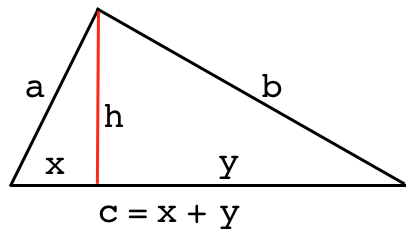
\includegraphics [scale=0.4] {triangle3.png} \end{center}

\[ a^2 - x^2 = h^2 \]
\[ b^2 - y^2 = h^2  \]

So
\[ a^2 = x^2 + h^2 = x^2 + b^2 - y^2 \]

But
\[ y = c - x \]
\[ y^2 = c^2 - 2cx + x^2 \]

Therefore:
\[ a^2 = x^2 + b^2 - (c^2 - 2cx + x^2) \]
\[ a^2 = b^2 - c^2 + 2cx  \]
Rearranging
\[ c^2 = a^2 + b^2 + 2cx  \]

Finally, $x = a \cos B$ so
\[ a^2 = b^2 - c^2 + 2ac \cos B  \]

This is the law of cosines.

$\square$

Any side of a triangle can be expressed in terms of the other two and the cosine of the angle between them.  Thus, for example
\[ c^2 = a^2 + b^2 - 2ab \cos C  \]
\[ a^2 = b^2 + c^2 - 2bc \cos A  \]

\subsection*{proof without words}
\begin{center} \includegraphics [scale=0.4] {law_of_cosines.png} \end{center}

Adding some words:

Draw a right triangle using one diagonal of a circle (any third point on the circle forms a right angle), then draw any other diagonal, in red.  

At the point of interest, the red diagonal is divided into $a + c$ and $a - c$.  The base of the black right triangle is $2a \cos \theta$ so it is divided into $b$ and $2a \cos \theta - b$.  

We apply the theorem on chords of a circle from (\hyperref[sec:chord_segments]{\textbf{here}}).  The products of the chord segments are equal.

\[ (a + c)(a - c) = (2a \cos \theta - b)(b) \]
\[ a^2 - c^2 = 2ab \cos \theta - b^2 \]
\[ c^2 = a^2 + b^2 - 2ab \cos \theta \]


\subsection*{Law of sines}
I'll just mention another identity called the law of sines.  In contrast to the law of cosines, it is fairly trivial to prove.
\begin{center} 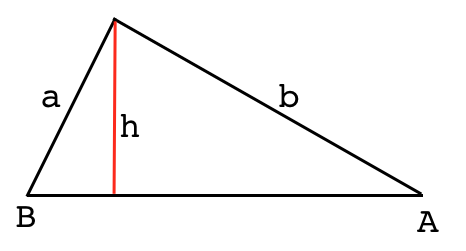
\includegraphics [scale=0.4] {triangle4.png} \end{center}

\[ \frac{h}{b} = \sin A \]
\[ \frac{h}{a} = \sin B \]
Therefore
\[ h = b \sin A = a \sin B \]
\[ \frac{\sin A}{a} = \frac{\sin B}{b} \]
We could do the same construction and argument with either $A$ or $B$, and the third angle, call it $C$.  Therefore
\[ \frac{\sin A}{a} = \frac{\sin B}{b} = \frac{\sin C}{c} \]

The sine of an angle, divided by the length of the side opposite, is a constant.

\end{document}